%************************************************
\chapter{Building blocks of a cross-platform Application}\label{ch:building}
%************************************************

When building a cross-platform applications, there are many aspects you need to plan, well before you start writing code. Thankfully we already know which framework we are going to use and are familiar with the programming language it uses. 

What we need to do now is analyze the requirements of the application, separate the business logic from the \ac{UI} logic, analyze third-party libraries that may speed up development and implement the application.


\section{Requirements for the MHM Job Portal Aggregator}
Every application needs a purpose. The main purpose of the \ac{JPA} is to consolidate open job vacancies from different sources into an easy to use mobile application. In order to fulfill this, we need to define some requirements of the functionality that the application should offer.  

\begin{description}
\item[Latest Jobs] The main window of the application should show the latest available vacancies, organized in a table view. Each cell should show the title of the vacancy, along with a short description and a small icon depicting the company from where the vacancy came.
\item[Detailed Description] A detailed description of the vacancy should appear when the user clicks on one of the table items. This view should include all the information about the job offering, including salary, benefits and how to apply.
\item[Offline Access] If there is no connection to the internet, the user should still be able to see the vacancies that were loaded the last time the application was opened.
\item[Social Integration] From the detailed description view, the user should be able to share a job offering with his friends via popular social networks like Facebook, Twitter or LinkedIn. 
\item[Search Functionality] Users should be able to search for vacancies based on keywords they enter on the search view. The results should be loaded every time the user changes the search string and the table view should be updated with the new results.
\item[Filters] Pre-defined filters should aid in the navigation of the available job offers.
\item[Saved Searches] The user should be able to save past searches and access them quickly at any time.   
\item[Notifications] The user can opt to receive notifications whenever a new vacancy matching previous searches is posted.
\end{description}

These are the basic requirements to get a functional application that is both useful and easy to use.

\autoref{fig:app_flow} on the following page shows a more detailed view of how the application workflow is supposed to work.

\begin{figure}
    \begin{center}
        {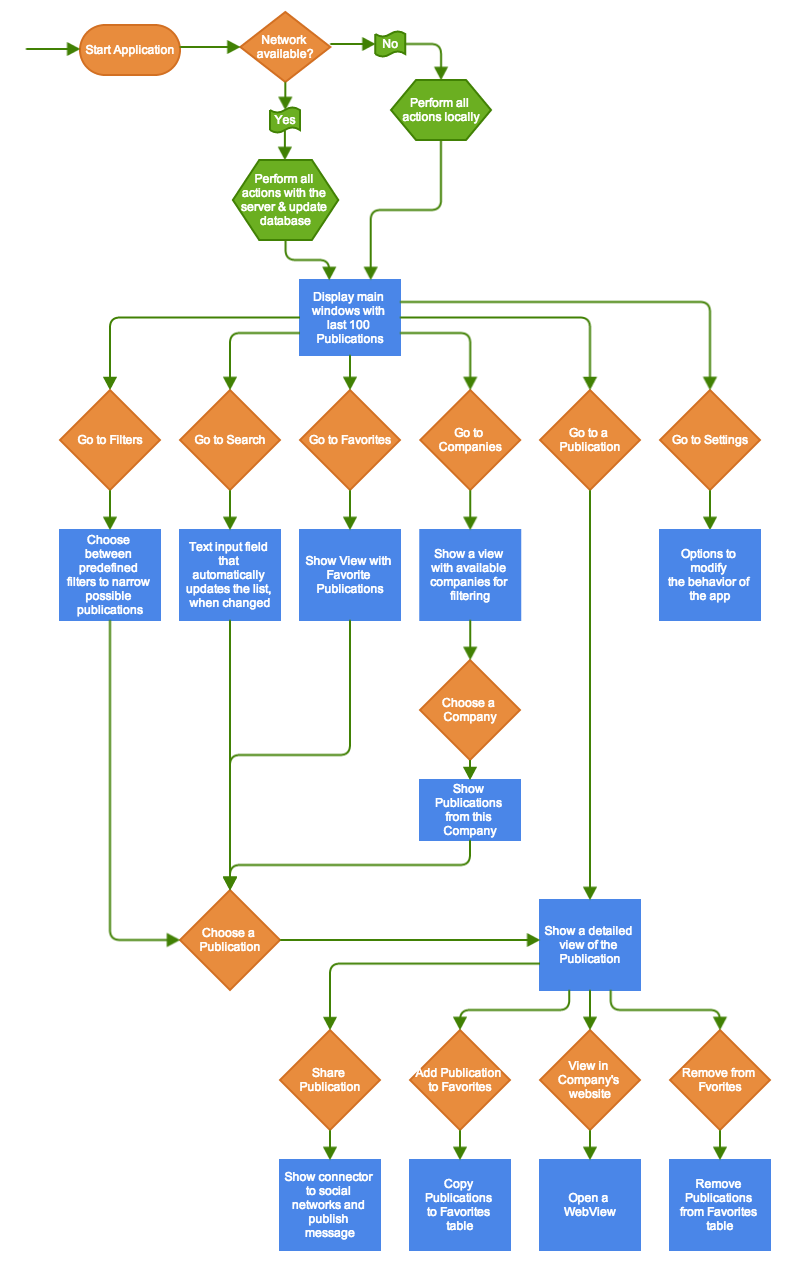
\includegraphics[width=1.14\linewidth]{gfx/app_flow}}
        \caption[Application Workflow]{Application Workflow}\label{fig:app_flow}
    \end{center}
\end{figure}



\section{Platform-Independent Functionality}

The building blocks of any application are mostly located within the business logic, even more so for cross-platform applications, since this is the layer where the shared code resides.

\subsection{Object Models \& Database Connections}
One of the easiest things to share between the platforms is the data handling code. There are two models we need in our application, \texttt{Publication} and \texttt{Company}.  

\texttt{Publications} represent each open vacancy that the application receives from the server and \texttt{Companies} represent each company offering those job applications and are there to help navigate the publications and filter them.

These objects not only represent an instance of the corresponding object in-memory, but, thanks to a third-party library called \textit{SQLite.NET}, they also represent the foundation of an \ac{ORM} System, that makes the creation and management of a local database much easier.

Normally, when using the platform specific SQLite implementation, you need to define the database, insert each element in the table and manage queries and updates manually. 

This can be really cumbersome if you have a lot of tables and elements in your database. By using \textit{SQLite.NET} there is no need for all these formalities, since the 'dirty' work is done by the library itself.
\vfill

\lstset{language=[Sharp]C}
\begin{lstlisting}[frame=lt,caption=Company.cs, label={list:comp}]
using SQLite;
namespace MHMBase
{
	[Table("companies")]
	public class Company
	{
		[PrimaryKey, AutoIncrement]
		public int Id { get; set; }
		[MaxLength(20)]
		public string Name { get; set; }
		public string FullName { get; set; }
		public string IconPath { get; set; }
		public string IconUrl { get; set; }
	}
}
\end{lstlisting}

\begin{lstlisting}[frame=lt,caption=Publication.cs, label={list:pub}]
using SQLite;
namespace MHMBase
{
	[Table ("publications")]
	public class Publication
	{
		[PrimaryKey, AutoIncrement]
		public int Id { get; set; }
		public string RemoteId { get; set; }
		[Indexed]
		public int CompanyId { get; set; }
		public string Title { get; set; }
		public string FullDescription { get; set; }
		public string Company { get; set; }
		[Unique]
		public string Link { get; set; }
		public string ShortDescription { get; set; }
		public bool Favorited { get; set; }
	}
}
\end{lstlisting}

\autoref{list:comp} and \autoref{list:pub} show us all the properties that we need for each model, and also give us a first hand look on how easy it is to use \textit{SQLite.NET}. All that is needed for models like this is to include an \texttt{Id} element with the default getters and setters preceded by the 'magic' attributes so often used in C\# that tell the \textit{SQLite.NET} constructors how to save and define each field in the database. 

\texttt{PrimaryKey} defines the following field as the primary entry of the database and \texttt{AutoIncrement} makes it increase in value, every time a new element is saved to the database. You can also specify the name of the table by adding \texttt{Table ("new-table-name")} before declaring the new class. If you don't specify this value, the table name will default to the class name.

There are many other identifiers that will modify this behavior and they share the same name as the normal SQL modifiers. Some of them are \texttt{Unique, MaxLength, Column}, etc. If you have a field that cannot be saved to the database, you can add the \texttt{Ignore} identifier so that \textit{SQLite.NET} will ignore this field when saving the object to the database.

But this is still just the starting point. We still ned to create an SQLite Connection, create the appropriate table for the objects, create a new object and insert it to the database. Thankfully this is a very easy and straightforward process.

\begin{lstlisting}[frame=lt,caption=DatabaseHelper.cs, label={list:db-save}]
using SQLite;
namespace MHMBase
{
	public class DatabaseHelper
	{
		static DatabaseHelper currentInstance;
		readonly SQLiteConnection db;
		public static DatabaseHelper Instance {
			get {
				if (currentInstance == null)
					currentInstance = new DatabaseHelper ();
				return currentInstance;			
			}
		}

		DatabaseHelper () {
			string folder = System.Environment.GetFolderPath (System.Environment.SpecialFolder.Personal);
			db = new SQLiteConnection (System.IO.Path.Combine (folder, "mhm-jpa.db"));		
		}

		public SQLiteConnection Connection {
			get { return db; }		
		}
	}
}
\end{lstlisting}

\autoref{list:db-save} gives us a first hand look of how we handle the Database Integration. The \texttt{DatabaseHelper} Singleton \marginpar{Singleton: Special Class that only allows for a single instance of itself.} is in charge of creating a single instance of an \texttt{SQLiteConnection} that will be used throughout both Android and iOS applications.

This \texttt{SQLiteConnection} instance is responsible for the management of everything related to the database. It is used to create or delete tables; add, edit or delete items; and to perform queries.

\begin{lstlisting}[frame=lt,caption=DB Snippet, label={list:db-snip}]
var db = DatabaseHelper.Instance.Connection;
// Create Companies Table
db.CreateTable<Company>();
// Create Company Object
var company = new Company {
                Name = "SuperComp",
                FullName = "Super Computers Inc.",
                IconPath = Path.Combine (Environment.GetFolderPath (Environment.SpecialFolder.Personal), "SuperComp.png"),
                IconUrl = "http://supercomp.com/icon"
            };
// Insert new element in DB
db.Insert(company);    
\end{lstlisting}

\autoref{list:db-snip} gives us a simple example of how to get the \texttt{SQLiteConnection} instance, create a table that will store \texttt{Company} objects, create a new object and save it to the database.

\begin{lstlisting}[frame=lt,caption=DB Snippet 2, label={list:db-snip2}]
//Get item by ID
var item = db.Get<Company>(3);
//Delete Item by ID
db.Delete<Company>(3);
//Return all objects in table
var allItems = db.Table<Company>();
//Select item via SQL Statement
var sc = db.Query<Company>("SELECT * FROM Companies WHERE Name = ?", "SuperComp");
//Get all items and order by Name
var companies = db.Table<Company>().OrderBy(c => c.Name);
//Update an object after it has been modified
db.Update(item);
\end{lstlisting}

\autoref{list:db-snip2}, on the other hand, shows us how we can access and manipulate existing objects on the database.

If it weren't for \textit{SQLite.NET} all of the code previously shown would be at least 3 times longer and more complex. Thanks to third-party libraries like this, we can keep our code cleaner and easier to maintain. We will discuss more about what third-party libraries we use later on.   

\subsection{Network Communications}
Another aspect of the application that is easy to share between platforms is the network access. We can easily use all the built in functionality of C\#'s standard library under \texttt{System.Net} and take advantage of asynchronous communication and \ac{LINQ} for \ac{XML} and \ac{JSON} parsing.

\begin{lstlisting}[frame=lt,caption=PublicationsParser.cs, label={list:db-pubparse}]
public void UpdatePublications(Action<IList<Publication>> callback, SQLiteConnection db) {
	db.CreateTable<Publication>();
	var client = new WebClient ();
	client.DownloadStringCompleted += (sender, args) => {
		var pubs = XDocument
		.Parse(args.Result)
		.Descendants("publication").Select(item => new Publication {
			RemoteId = item.Element("id").Value,
			Title = item.Element("title").Value,
			[...]
		}).ToList();
		foreach (var p in pubs) {
			try {
				db.Insert (p);
			} catch (SQLiteException){
				Console.WriteLine ("Duplicate detected");
			}				
		}
		callback(GetPublications(db));
	};
	client.DownloadStringAsync (new Uri (_baseUrl));
}
\end{lstlisting}

A deeper look at \autoref{list:db-pubparse} shows that \texttt{UpdatePublications} method is in charge of fetching the latest \texttt{Publications} and updating the database with the new information. Let's break it apart to see exactly how it works.

The method takes two arguments: a callback action to be executed when the asynchronous download finishes and a reference to an \texttt{SQLiteConnection} object that will update the database.

Once the method starts executing it will create a the \texttt{Publication} table if it doesn't exist already and create an instance of a \texttt{WebClient}. The Web Client does all the heavy lifting and takes care of connecting to the server. The connection is done asynchronously, so we need to define the \texttt{DownloadStringCompleted} method that gets executed once the download of data has completed.

Inside this method lives the code that actually takes care of parsing the \ac{XML} file and saving the new Publications to the database. Thanks to \ac{LINQ}, iterating over each element inside the \ac{XML} file is fairly easy. All we need is an \texttt{XDocument} object to parse the results and iterate over the descendants inside the \ac{XML} tree that match the "publication" tag, then the \texttt{Select} method is called for each item passing a lambda function that makes use of this item and creates a new \texttt{Publication} object. Once everything is done, everything gets thrown into a list and saved to the \texttt{pubs} variable. 

Now that we have a list containing \texttt{Publication} objects we can add them to the database. After everything is saved, we can call the \texttt{callback} function passing as argument the \texttt{GetPublications} function that simply retrieves all elements inside the \texttt{Publications} table.

How the \texttt{callback} functions are used and what they do, we will learn later on.

\begin{lstlisting}[frame=lt,caption=CompaniesParser.cs,label={list:db-compparse}]
foreach (var c in companies) {
	try {
		db.Insert (c);
		var webClient = new WebClient();
		var url = new Uri (c.IconUrl);
		var image_bytes = webClient.DownloadData (url);
		string documentsPath = Environment.GetFolderPath (Environment.SpecialFolder.Personal);	
		string localPath = Path.Combine (documentsPath, c.Name+".png");
		Console.WriteLine("localPath:"+localPath);
		File.WriteAllBytes (localPath, image_bytes);		
	} catch (SQLiteException) {
		Console.WriteLine ("Duplicate detected");					
	}
}
\end{lstlisting}

This process for retrieving the available companies is very similar, almost identical, so we will only take a look at the part that is different. Once everything has been downloaded, parsed and stored in a list, we iterate over this list and if the object doesn't exist in the database, we save it and then download an icon for the logo of this company to the internal storage, so that it can be retrieved by each publication belonging to this company. The code for this can be seen in \autoref{list:db-compparse}.

\section{Third-Party Libraries}

As we mentioned before, third-party libraries are a great way of speeding up development, lowering complexity and improving maintainability. We already talked about one of this libraries, \textit{SQLite.NET}, and how we use it in our application. The following are all the libraries we use that are compatible with both platforms. 

\subsection{Newtonsoft JSON}

As the name implies, \textit{Newtonsoft JSON} is a library designed for parsing \ac{JSON} strings. It has built-in support for \ac{LINQ}, making deserialization much simpler and also supports \ac{XML} to \ac{JSON} conversion.

Inside our application we use it to deserialize the returned result string, when the user preforms a search.

Thanks to \ac{LINQ}, the code in charge of deserializing each element is very similar to the \ac{XML} deserialization code.

\begin{lstlisting}[frame=lt,caption=Publication Search,label={list:search}]
public void SendSearchParameters(Action<IList<Publication>> callback, string parameters) {
	var dl = new WebClient();
	dl.Headers.Add("Content-Type","application/json");
	dl.UploadStringCompleted += (sender, e) => {
		var resultJSON = JObject.Parse (e.Result);
		IList<Publication> publications = resultJSON["publications"].Select(item => new Publication	{
			RemoteId = (string)item["id"],
			Title = (string)item["title"],
			[...]				
		}).ToList();
		callback(publications);
	};
	dl.UploadStringAsync (new Uri (_searchUrl), parameters);		
}
\end{lstlisting}

As \autoref{list:search} shows, we again need a \texttt{WebClient} that takes care of uploading the search parameters to the server and that registers an \texttt{UploadStringCompleted} method that gets executed once the uploading has finished.

Once we have the result string, it gets parsed by the \texttt{JObject} class from \textit{Newtonsoft JSON}. This creates a \texttt{JObject} that is composed of a \texttt{Collection} of \texttt{JTokens}, each representing a serialized element of the result string. We can then access each item inside the "publications" token via \ac{LINQ} with the \texttt{Select} function and create a \texttt{Publication} object out of each item. All of these \texttt{Publication} objects get packed in a list and then passed to the \texttt{callback} function.

The \textit{Newtonsoft JSON} library makes the serialization and deserialization of objects easier and faster. If the \ac{JSON} structure matches the structure of a C\# object, this library can deserialize it and create a new object, without the need to manually match each \ac{JSON} element to an object attribute.
 

\subsection{SimpleStorage}
\textit{SimpleStorage} is a very straight forward third-party library that makes the storing of key-value paired data as easy as possible. It exposes a platform-independent \ac{API} that utilizes each platforms's preferences storage, so you don't need to worry about the implementation in each platform and can share your storage saving code between them.

\begin{lstlisting}[frame=lt,caption=SimpleStorage,label={list:store}]
var storage = SimpleStorage.EditGroup("group name");
storage.Put("myKey", "some value");
var value = storage.Get("myKey");
\end{lstlisting}

We use this library to store simple settings and execution states.


\subsection{SQLite.NET}
We already discussed most of the functionality of \textit{SQLite.NET} in a previous section, so there is not that much to talk about, except for some features that we don't use in our application.

\textit{SQLite.NET} features an asynchronous \ac{API} that doesn't block the main thread while running, thus allowing the rest of the application to continue executing as normal, while the SQL request are performed in the background. The functionality of the library remains the same and the only thing that is different are the method signatures. For example, instead of calling \texttt{CreateTable<T>}, you call \texttt{CreateTableAsync<T>} to create a new table, so all that is needed is to add \texttt{Async} at the end of each method call to use the asynchronous \ac{API}.

\textit{SQLite.NET} also has support for transactions. You can execute database operations inside a transaction and, if something were to fail, the database would be rolled back to the point before the transaction started.

You can also create relationships between objects by adding the \texttt{Indexed} attribute to any model. Going from our application we have the \texttt{CompanyId} field in our \texttt{Publication} model with the \texttt{Indexed} attribute. What this does is















